\documentclass[conference]{IEEEtran}

% ===== Packages =====
\usepackage{graphicx}
\usepackage{amsmath}
\usepackage{siunitx}
\usepackage{cite}
\usepackage{tikz}
\usetikzlibrary{arrows.meta,positioning,fit,calc,shapes.geometric,decorations.pathreplacing}
\usepackage[hidelinks]{hyperref}
\urlstyle{same}

% ===== Title & Author =====
\title{Lead-free Bio-Inkjet Printing with Bulk KNN Actuators and AITL-based Adaptive Control}

\author{
  \IEEEauthorblockN{Shinichi Samizo}
  \IEEEauthorblockA{Independent Semiconductor Researcher\\
  Former Engineer at Seiko Epson Corporation\\
  Email: \href{mailto:shin3t72@gmail.com}{shin3t72@gmail.com}\\
  GitHub: \url{https://github.com/Samizo-AITL}}
}

\begin{document}
\maketitle

% ===== Abstract =====
\begin{abstract}
This paper proposes a biocompatible inkjet printing architecture based on
lead-free piezoelectric actuators, specifically bulk KNN (K,Na)NbO$_3$, combined
with chip-on-film (COF) driver ICs, silicon cavity integration, and
an AITL (Adaptive Intelligent Three-Layer) supervisory control framework.
Unlike conventional PZT-driven industrial heads, the KNN approach supports
biocompatibility and Pb-free compliance, while moderate performance
(3--5 pL droplets, $10^6$ shots, $\pm50$ V operation) satisfies bioprinting needs.
Beyond actuation, the electromechanical response of KNN is leveraged for
\emph{self-diagnosis}: detecting missing droplets and estimating ink viscosity.
This diagnostic data feeds into an AITL architecture---an inner PID loop for
real-time stability, an FSM layer for mode transitions and compensation,
and an LLM-driven supervisory layer for adaptive redesign of control rules.
We present the architecture, process flow, and representative biomedical
applications, highlighting the potential of KNN as both actuator and sensor.
\end{abstract}

% ===== Sections =====
\section{Introduction}
% sections/intro.tex

\section{Introduction}

Memory hierarchies are central to computing systems. 
DRAM remains the dominant volatile memory due to speed, density, and scalability \cite{choi2022,kim2021_dram}. 
However, DRAM scaling faces limits as capacitors shrink; 3D DRAM concepts are explored to extend scaling \cite{iedm2023_dram}.

In parallel, doped HfO$_2$ ferroelectrics enabled FeRAM and FeFET with CMOS-friendly integration \cite{boscke2011,mueller2012}. 
These offer non-volatility with fast switching but face polarization variability, endurance, and TDDB concerns. 

This review contrasts DRAM and FeRAM at device and system levels and outlines hybrid use-cases. 
As an overview, Figs.~\ref{fig:speed_retention} and \ref{fig:energy_speed} conceptually illustrate the trade-offs in access speed, retention, and write energy, which will be detailed in Sec.~\ref{sec:comparison}.


\section{Background: Pb-free Piezoelectrics}
\section{Background}
This work builds on the author's 1997–1998 ramp activities at Epson's Sakata fab under technology transfer from Mitsubishi; details are summarized in the Introduction and referenced archives.


\section{Proposed Bio-IJ Architecture}
\section{Proposed Architecture}
The proposed Bio-Inkjet (Bio-IJ) actuator system is designed to balance
biocompatibility, manufacturability, and sufficient actuation
performance for biomedical applications. Its main components are as
follows:
\begin{itemize}
  \item \textbf{Bulk KNN multilayer stack actuator}:
        A 200--500~\si{\micro\meter} thick piezoelectric stack providing
        moderate displacement suitable for picoliter-scale droplet
        ejection.
  \item \textbf{COF driver IC}:
        A chip-on-film high-voltage driver with 16--32 channels,
        operating at up to $\pm 50$~\si{\volt}, and incorporating waveform RAM
        with SPI control for flexible pulse shaping.
  \item \textbf{Si cavity and nozzle array}:
        A silicon-etched cavity directly bonded to the actuator, with
        nozzles of $\varphi$\SI{8}{\micro\meter} diameter producing
        droplets in the 3--5~\si{\pico\liter} range.
  \item \textbf{Reservoir and back pressure control}:
        A fluidic supply stabilized at approximately $-2.0$~kPa using
        a PID-controlled regulator to ensure consistent meniscus
        positioning.
  \item \textbf{PI membrane damper}:
        A polyimide-based damping layer integrated in the reservoir to
        suppress pressure fluctuations and prevent satellite droplets.
\end{itemize}

The associated \textit{process flow} begins with fabrication of the bulk
KNN stack and electrode finishing, followed by terminal cutting and COF
assembly. The actuator is then mounted with a heat spreader for thermal
management and finally bonded to the silicon cavity structure,
resulting in an integrated Bio-IJ printhead module.

% ===== Figures (1-column) =====

% Fig.1: Block diagram (vertical layout to fit one column)
\begin{figure}[t]
  \centering
  \tikzset{font=\footnotesize}
  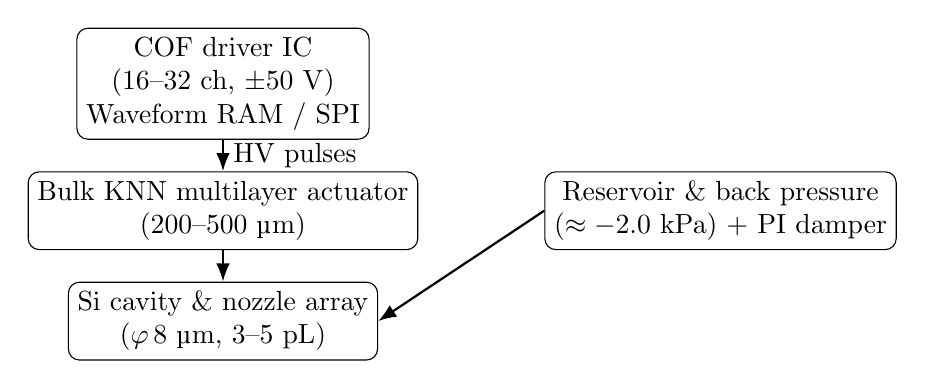
\begin{tikzpicture}[
      node distance=4mm and 6mm,
      box/.style={draw, rounded corners, align=center, minimum width=34mm, minimum height=7mm},
      arrow/.style={-Latex, thick}
    ]
    % Nodes (vertical stacking)
    \node[box] (cof) {COF driver IC\\(16--32 ch, $\pm 50$~\si{\volt})\\Waveform RAM / SPI};
    \node[box, below=of cof] (knn) {Bulk KNN multilayer actuator\\(200--500~\si{\micro\meter})};
    \node[box, below=of knn] (noz) {Si cavity \& nozzle array\\($\varphi$\,8~\si{\micro\meter}, 3--5~\si{\pico\liter})};
    \node[box, right=16mm of knn] (bp) {Reservoir \& back pressure\\($\approx -2.0$~kPa) + PI damper};

    % Arrows
    \draw[arrow] (cof) -- node[right]{HV pulses} (knn);
    \draw[arrow] (knn) -- (noz);
    \draw[arrow] (bp.west) -- (noz.east);
  \end{tikzpicture}
  \caption{System architecture of the proposed Bio-Inkjet (Bio-IJ). A bulk KNN actuator, COF high-voltage driver, silicon cavity/nozzles, and fluidics (back-pressure with PI damper) are integrated.}
  \label{fig:block}
\end{figure}

% --- Fig.2: Cross section (single-column width, 上部説明をさらに上へ) ---
\begin{figure}[!t]
  \centering
  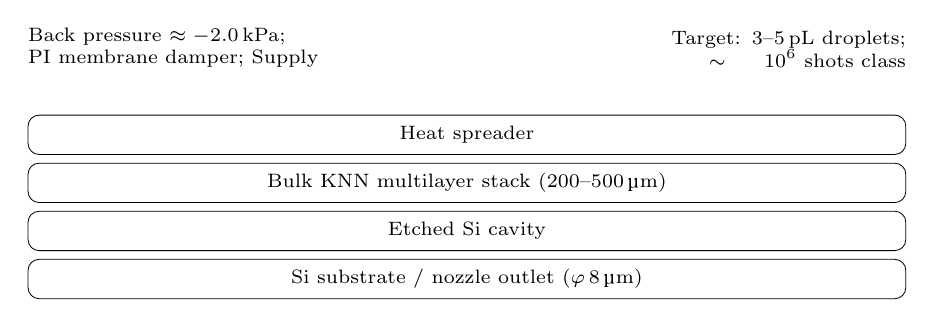
\begin{tikzpicture}[
      every node/.style={font=\scriptsize},
      box/.style={draw, rounded corners, align=center,
                  minimum height=5mm, text width=.90\linewidth},
      line width=0.3pt
    ]
    % 本体レイヤ
    \node[box] (hs)  {Heat spreader};
    \node[box, below=1mm of hs]  (act) {Bulk KNN multilayer stack (200--500\,\si{\micro\meter})};
    \node[box, below=1mm of act] (cav) {Etched Si cavity};
    \node[box, below=1mm of cav] (sub) {Si substrate / nozzle outlet ($\varphi$\,8\,\si{\micro\meter})};

    % ── 上部説明(さらに上にシフトして重なり解消) ──
    \node[align=left, anchor=south west, text width=.44\linewidth, inner sep=0pt]
      at ([yshift=6mm]hs.north west)
      {Back pressure $\approx -2.0$\,kPa;\\ PI membrane damper; Supply};

    \node[align=right, anchor=south east, text width=.44\linewidth, inner sep=0pt]
      at ([yshift=6mm]hs.north east)
      {Target: 3--5\,\si{\pico\liter} droplets;\\ $\sim 10^6$ shots class};
  \end{tikzpicture}
  \caption{Cross-sectional schematic of the Bio-IJ printhead.
  The KNN stack is bonded to a silicon cavity with $\varphi$\,8\,\si{\micro\meter}
  nozzles; fluidics provide back-pressure stabilization and damping.}
  \label{fig:section}
\end{figure}


\section{Self-Diagnosis and Feedback Control}
The bulk KNN actuator can also function as a proxy sensor by monitoring
its electromechanical response during drive pulses.
\subsection{Dot-Missing Detection and Compensation}
By observing charge/displacement signatures, missing droplets are detected
without external optics. An FSM controller triggers neighboring-nozzle
compensation, preserving array-level print reliability.
\subsection{Viscosity Estimation and Drive Adaptation}
Viscosity changes appear as altered dynamic response.
The PID loop adjusts drive voltage/pulsewidth in real time.
This closes the loop between fluid rheology and actuator operation.

\section{AITL Control Framework}
The Adaptive Intelligent Three-Layer (AITL) framework integrates:
\begin{itemize}
\item \textbf{Inner PID}: ensures real-time stability of droplet ejection.
\item \textbf{Intermediate FSM}: supervises nozzle states, detects anomalies,
and switches modes (normal, compensation, cleaning).
\item \textbf{Outer LLM}: analyzes long-term trends, re-identifies PID gains,
and redefines FSM transitions when performance degrades.
\end{itemize}
A schematic is shown in Fig.~\ref{fig:aitl}.
\begin{figure}[t]
\centering
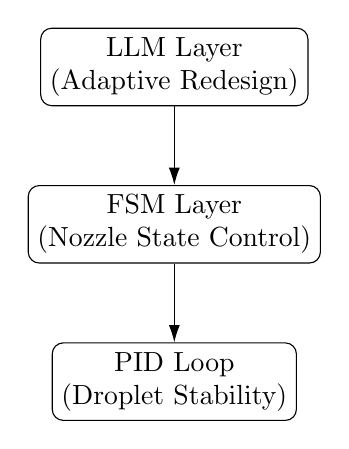
\begin{tikzpicture}[
  block/.style={draw, rounded corners, minimum width=2.4cm, minimum height=8mm, align=center},
  line/.style={-{Latex[length=2.2mm,width=1.4mm]}}
]
\node[block] (pid) {PID Loop\\(Droplet Stability)};
\node[block, above=of pid] (fsm) {FSM Layer\\(Nozzle State Control)};
\node[block, above=of fsm] (llm) {LLM Layer\\(Adaptive Redesign)};
\draw[line] (fsm) -- (pid);
\draw[line] (llm) -- (fsm);
\end{tikzpicture}
\caption{AITL three-layer architecture for Bio-IJ adaptive control.}
\label{fig:aitl}
\end{figure}

\section{Applications}
\section{Applications}
The proposed Bio-Inkjet architecture enables several key biomedical
applications in which moderate actuation performance, precise droplet
control, and biocompatibility are prioritized over extreme durability:
\begin{itemize}
  \item \textbf{Cell patterning}: 
        Controlled deposition of living cells into predefined patterns
        for tissue engineering and regenerative medicine.
        Gentle actuation and droplet volumes of 1--10~\si{\pico\liter}
        support high cell viability, with survival rates above 80\%
        reported under comparable shear stress conditions.
  \item \textbf{Protein and DNA microarrays}: 
        Picoliter-scale dispensing of biomolecules onto functionalized
        substrates for high-throughput screening, diagnostics, and
        drug discovery.
        The ability to generate uniform, sub-100~\si{\micro\meter}
        spots is critical for assay reproducibility.
  \item \textbf{Hydrogel 3D printing}: 
        Layer-by-layer deposition of bio-compatible hydrogels, followed
        by UV or thermal curing, to fabricate soft scaffolds for cell
        culture and organ-on-chip platforms.
        Precise droplet placement ensures structural fidelity and
        material homogeneity.
\end{itemize}

These use cases demonstrate that the moderate performance of bulk KNN
actuators---picoliter droplet generation at voltages below
$\pm 50$~V---is sufficient to meet biomedical requirements.
Here, droplet volume control, biocompatibility, and integration with
fluidic handling systems are far more critical than the billion-cycle
endurance demanded in industrial printing.


\section{Conclusion}
% sections/conclusion.tex

DRAM will continue to dominate volatile working memory due to speed, density, and ecosystem maturity. HfO2-based FeRAM/FeFET offers a CMOS-compatible non-volatile complement with fast access, though variability, endurance dispersion, and integration limits remain active topics \cite{noheda2023,martin2020}. Hybrid hierarchies that pair DRAM for hot data with FeRAM for persistence can reduce refresh energy while enabling fast recovery paths.

Looking ahead, co-design across devices, controllers, and operating systems will be central: retention-aware placement, telemetry-driven reliability management, and low-latency persistence paths are promising directions to broaden deployment from embedded and edge to selected data-centric systems.


% ===== References =====
\nocite{Saito2004KNN,Dubois2019BioIJ}
\bibliographystyle{IEEEtran}
\bibliography{refs}

% ===== Biography =====
\section*{Author Biography}
\textbf{Shinichi Samizo} received the M.S. degree in Electrical and Electronic
Engineering from Shinshu University, Japan. He worked at Seiko Epson
Corporation as an engineer in semiconductor memory and mixed-signal
device development, and contributed to inkjet MEMS actuators and
PrecisionCore printhead technology. He is currently an independent
semiconductor researcher focusing on process/device education, memory
architecture, and AI system integration. Contact:
\href{mailto:shin3t72@gmail.com}{shin3t72@gmail.com}.
\end{document}
